\documentclass[11pt]{article}
\usepackage[utf8]{inputenc}
\usepackage[T1]{fontenc}
\usepackage[brazil]{babel}
\usepackage{newtxtext} % Times New Roman
\usepackage[top=3cm, bottom=2cm, left=3cm, right=2cm]{geometry}
\usepackage{ragged2e}
\usepackage{enumitem}
\usepackage{setspace}
\usepackage{makeidx}
\usepackage{graphicx}
\usepackage{afterpage}
\usepackage{booktabs}
\makeindex % Criar índice depois


% Início do corpo do texto
\begin{document}

\justifying % Texto justificado
\onehalfspacing % Espaçamento de 1,5 linha
\setlength{\parindent}{0cm}  % Indentação dos parágrafos
\renewcommand*\familydefault{\rmdefault}
%-----------------------------------------------------------%
% Capa                                
%-----------------------------------------------------------%
\thispagestyle{empty}
\begin{center}

\includegraphics[scale=0.6]{capa/logo-dep.jpg}\\
\vspace*{.8cm}
{\huge \textbf{UNIVERSIDADE FEDERAL DE SÃO CARLOS}}\\
\vspace*{.8cm}
{\Larsge \textbf{SIMULAÇÃO DE SISTEMAS}}\\s
\vspace*{3cm}
{\Large \textbf{ANÁLISE DE DADOS HISTÓRICOS DE UM CALL CENTER}}\\
\vspace*{4.5cm}
\begin{flushright}
    \onehalfspacing
    {\Large  Paulo Roberto Mattielo Filho - 792323}\\
    {\Large  Pedro Peverari Di Lallo - 792328}\\
    {\Large  Lucas Gabriel Malheiros - 769837}\\
    {\Large  Vinícius Nobre - }\\
    \vspace*{.3cm}
    {\Large \textbf{Professor:}}
    {\Large VCBC}\\
\end{flushright}
\vspace*{\fill}
{\large \bf SÃO CARLOS / 2023}
\end{center}



\newpage{}
\tableofcontents{}
\newpage{}

\section{Introdução}
\subsection{Descrição do problema}
ESCREVER UMA DESCRIÇÃO (PRA VALER) DO PROBLEMA DO CALL-CENTER E QUAIS QUESTÕES VAMOS ABORDAR.

\subsection{Alterações da versão anterior}
Descrição mais detalhada do problema da central de atendimentos.\\
Os gráficos de linhas das Figuras \ref*{fig: chamados-tempo}, \ref*{fig: t_servico-tempo}, \ref*{fig: espera-tempo} e \ref*{fig: arrivals-tempo} foram substituídos por gráficos de dispersão.\\
A Figura \ref*{fig: correlogram} foi adicionada ao estudo de correlação das variáveis na Seção \ref*{section: correlacao-anual} para auxiliar na visualização do resultado obtido pelo teste de correlação de Spearman.\\
As seções de introdução e conclusão foram reorganizadas para a escrita de novos conteúdos.\\
Realização dos testes de aderência mensais para tempos entre chegadas na Seção \ref*{section: fit-arrivals}.\\
Correção de erros gerais de redação e referências.



\section{Análise de dados}
\subsection{Análise anual}
Inicialmente, foram levantadas as quantidades de ligações registradas durante o ano e a quantidade total de falhas, assim como o percentual de falhas. No ano de 2021, que contou com 261 dias de trabalho, foram registradas 51.708 ligações, sendo que 4.227 destas demoraram mais de 60 segundos para serem atendidas, caracterizando falha do processo. O percentual destas falhas para o ano foi de 8,17\%, valor que atende as especificações de desempenho da empresa. No entanto, como este valor representa apenas uma média anual, devemos buscar compreender o problema da empresa ao avaliar o comportamento das variáveis relevantes do processo ao longo do ano.

\subsubsection{Quantidade de chamados por dia}
A Figura \ref*{fig: chamados-tempo} apresenta a quantidade de chamadas recebidas por dia ao longo do ano. É possível perceber uma relação de dependência entre a quantidade de ligações recebidas e os dias do ano, visto que o número de chamadas cresce ao longo do ano. Esse comportamento pode ser responsável pelo aumento do percentual de falhas em meses próximos ao fim do ano. Posteriormente, será descrito um estudo de regressão para estes dados.

\begin{figure}[h]
    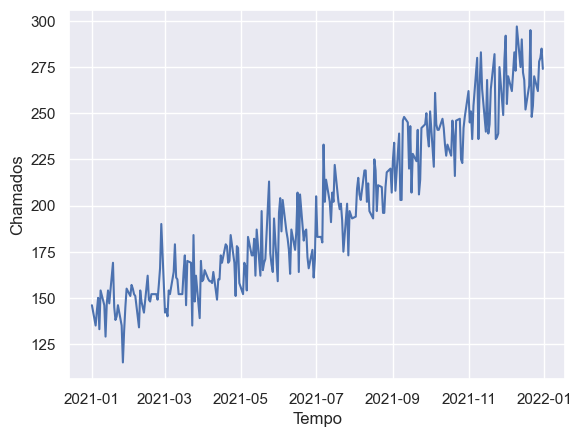
\includegraphics{analise-de-dados/anual/chamados.png}
    \caption{Quantidade de chamadas recebidas ao longo do tempo}
    \label{fig: chamados-tempo}
\end{figure}

\subsubsection{Análise e descrição dos tempos de espera e serviço}
Como os tempos de espera (\textit{wait length}) e serviço (\textit{service length}) já estão calculados, podemos analisar seu comportamento.

\begin{table}
\centering
    \begin{tabular}{lr}
        % \begin{center}
            \toprule
            {} &  Tempo de espera \\
            \midrule
            count &   51708.000  \\
            mean  &      17.035  \\
            std   &      64.061  \\
            min   &       0.000  \\
            25\%   &       0.000  \\
            50\%   &       0.000  \\
            75\%   &       0.000  \\
            max   &     983.000  \\
        % \end{center}
        \bottomrule
        % \label{tab: describe-wait}
    \end{tabular}
\caption{Estatística descritiva dos tempos de espera}
\label{tab: descricao-espera}
\end{table}

Teste

\subsection{Análise mensal}
Foi realizada uma agregação mensal a fim de visualizar as tendências das variáveis do sistema estudado ao longo do ano. Para isso, foi gerada uma tabela com um resumo das médias dos tempos de espera, serviço e de tempo entre chegadas das ligações mês a mês.\\
A partir disso, foi possível calcular a porcentagem de falhas ("\%\_failure") com base na divisão do número total de ligações que demoraram mais de 60 segundos para serem atendidas pelo total de ligações atendidas em cada mês.\\
A partir da Figura \ref*{fig: tmes} é possível visualizar alguns dados relevantes e transformar a base de dados com filtro mês a mês em informações capazes de nos demonstrar o comportamento do processo de atendimento nos quesitos tempo de espera médio, duração média do atendimento, média do tempo entre as chegadas, média do número de ligações recebidas e também a porcentagem de falhas.  

\begin{figure}[H]
    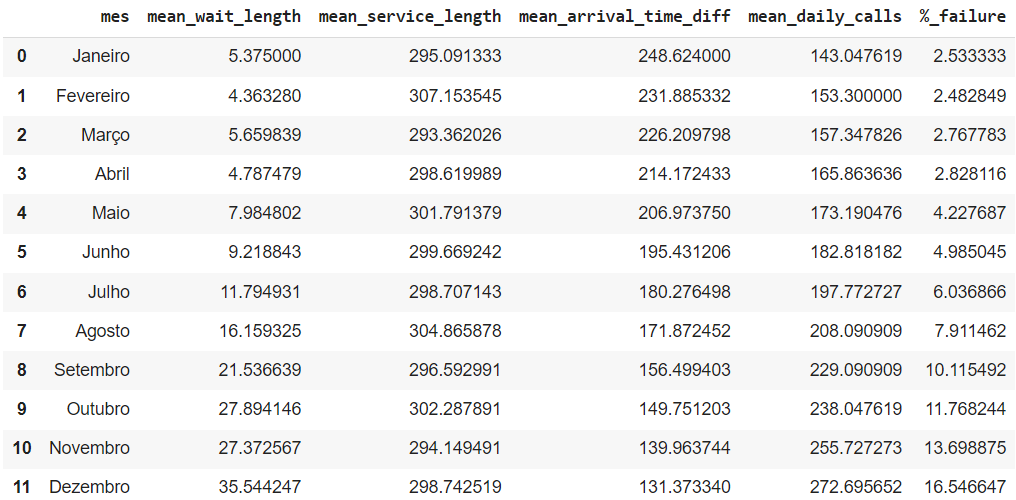
\includegraphics[scale=0.75]{analise-de-dados/mensal/tabmens.png}
    \caption{Tabela de resumo das médias dos tempos de espera, serviço e de chegada de ligações mês a mês}
    \label{fig: tmes}
\end{figure}

Realizando uma análise de cada uma das variáveis do sistema, apoiando-se nos testes de hipótese realizados anteriormente, é possível obter as seguintes conclusões a respeito dessas variáveis:
\begin{itemize}
    \item Tempo de espera: aumenta mês a mês;
    \item Média do tempo de serviço: relativamente constantes;
    \item Tempo entre chegadas: diminui mensalmente;
    \item Número de ligações: aumenta mensalmente;
    \item Percentual de falhas: aumenta mês a mês. A partir de setembro de 2021, a tolerância de 10\% que foi estipulada pelo
     gerente é superada.\\
\end{itemize}

Portanto, o percentual de falhas, aqui definido como o percentual de chamadas que demoram mais de 60 segundos para serem atendidas, aumenta mês a mês, ultrapassando, a partir de setembro de 2021,
a tolerância de 10\% necessária para cumprir a meta de desempenho de 90\% das chamadas atendidas em até 1 minuto.
\subsection{Análise trimestral}
Agregando os valores para períodos trimestrais conseguimos chegar aos dados presentes na Tabela \ref*{fig: tritab_img}:

\begin{figure}[H]
    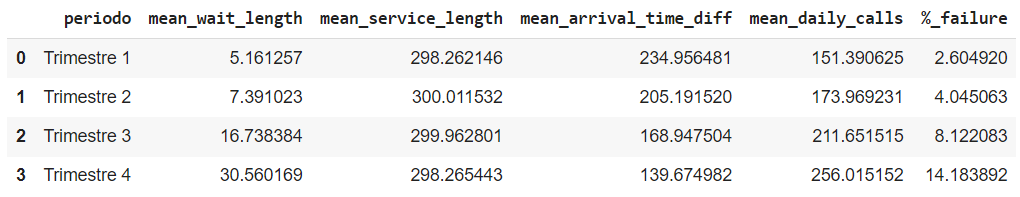
\includegraphics[scale=0.7]{analise-de-dados/trimestral/tritab.png}
    \caption{Tabela de resumo das médias dos tempos de espera, serviço e de chegada de ligações mês a mês}
    \label{fig: tritab_img}
\end{figure}

Tal análise trimestral acaba subestimando a porcentagem de falhas e acaba ocultando algumas informações como a falha no mês de setembro, que está no terceiro trimestre e passa a estar fora da zona de falha estipulada pela gerência.\\
Além disso, também é notável que o caminho correto não é agregar o intervalo de chegadas em períodos ainda maiores, como no trimestre, já que este é um valor alterado mensalmente.\\
Por fim, é possível observar que algumas conclusões semelhantes serão alcançadas em uma análise de cada uma das variáveis, no entanto, há uma perda de informações relevantes, não sendo a melhor maneira de observar o processo.\\
\subsection{Análise semanal}
O ponto principal para a escolha ou não da análise semanal é justamente a existência de diferenças das amostras semanais entre si, que justificaria posterior análise dos dados para melhor compreensão.\\
\subsubsection{Análise dos tempos de espera e serviço}
O teste não paramétrico de Kolgomorov Smirnov novamente foi utilizado para realização do teste de hipótese.\\
Para que não houvesse uma matriz com as respostas desnecessariamente grande (matriz 52x52) foi realizado o teste apenas para as semanas dos meses de dezembro e janeiro.\\
\begin{center}
    \begin{figure}[H]
        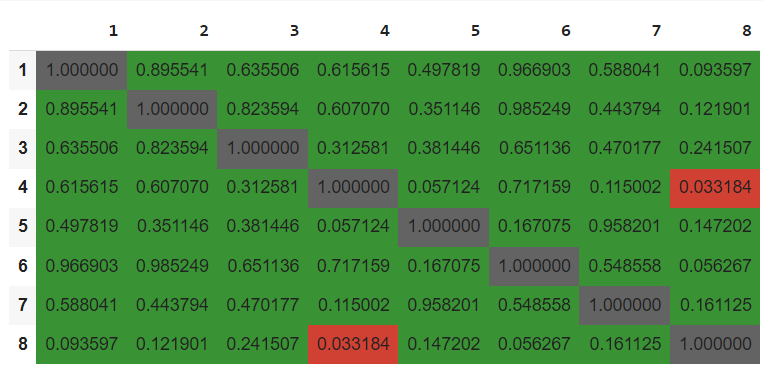
\includegraphics{analise-de-dados/semanal/janas.png}
        \caption{Kolgomorov Smirnov - teste para intervalos de chegada nas semanas de janeiro}
        \label{fig: jan_as_img}
    \end{figure}
    \begin{figure}[H]
        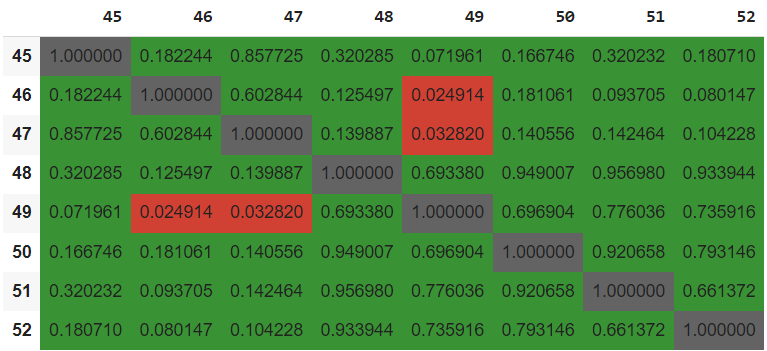
\includegraphics{analise-de-dados/semanal/dezas.png}
        \caption{Kolgomorov Smirnov - teste para intervalos de chegada nas semanas de dezembro}
        \label{fig: dez_as_img}
    \end{figure}
\end{center}
A figura \ref*{fig: jan_as_img} realiza o teste para os tempos de intervalo de chegada no mês de janeiro\\
A figura \ref*{fig: dez_as_img} realiza o teste para os tempos de intervalo de chegada no mês de dezembro\\
Foi possível observar que no horizonte de planejamento semanal, semanas subsequentes tendem a ter intervalos de chegada que seguem a mesma distribuição de probabilidade e, portanto, o planejamento semanal não é interessante para esse problema, visto que não é possível perceber as diferenças de demanda nesse nível de análise.
\subsection{Estudos de Regressão}

Ao montarmos a visualização dos tempos de chegada ao longo do tempo percebemos que havia tendência nos dados. Para isso, primeiro, calculamos todos os tempos de chegada das chamadas, subtraindo o horário de recebimento de uma chamada subsequente pelo da anterior, isto é:

$$Tempo_{chegada}(c_n) = t_n - t_{n-1}$$ 


Depois, as chamadas foram classificadas por dia, e, assim, calculado o tempo de chegada médio diário delas. O principal intuito desta etapa é facilitar a visualização da evolução desse parâmetro ao longo do tempo. O gráfico obtido por essa operação está abaixo, na figura 13.

\begin{figure}[H]
    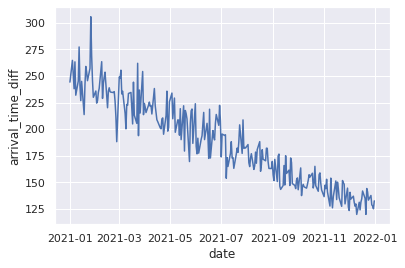
\includegraphics{analise-de-dados/regressao/tempo_chegada_medio.png}
    \caption{Tempo médio de chegada ao longo do Ano}
    \label{fig: tempos_de_chegada}
\end{figure}

A partir dessa percepção, são, então, propostos alguns estudos de regressão mais particulares para representar a tendência dos dados. Um usando "Ordinary Least Squares" e uma regressão exponencial.  

\subsection{Ordinary Least Squares}

Utilizando a biblioteca statsmodel do python foi realizado o estudo de regressão. A Equação Obtida foi: $$intervalos(t) = -0,4933 \cdot t + 252,6629$$. O resumo da regressão e o plot podem ser colocados a seguir: 

\begin{figure}[H]
    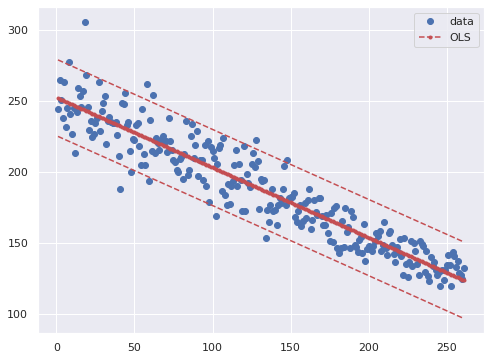
\includegraphics{analise-de-dados/regressao/regressao_OLS.png}
    \caption{Regressão Linear para os tempos de espera}
    \label{fig: plot_OLS}
\end{figure}

\begin{figure}[H]
    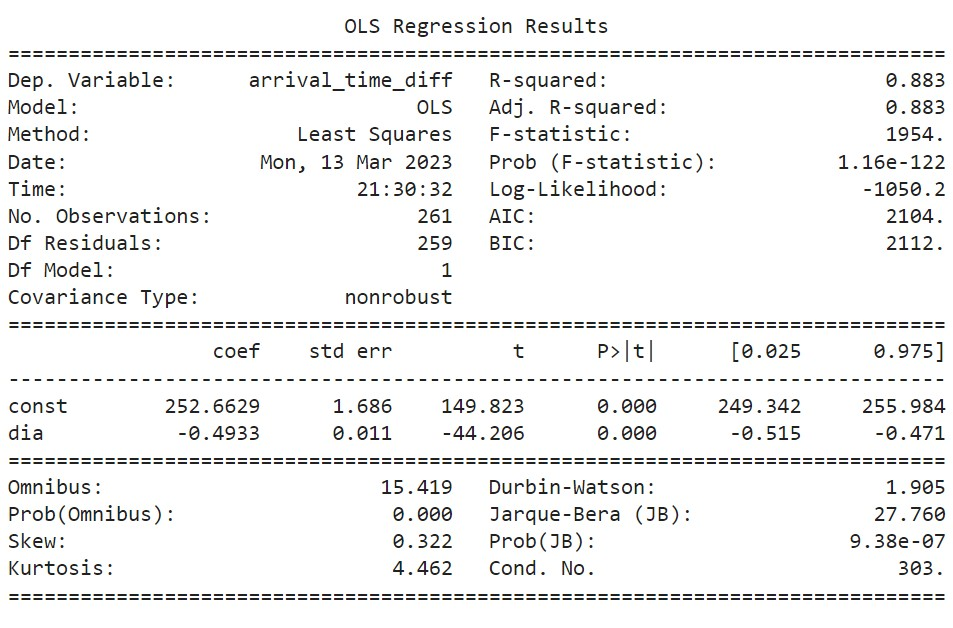
\includegraphics[scale = 0.85]{analise-de-dados/regressao/OLS_summary.jpg}
    \caption{Resumo da regressão}
    \label{fig: sum_OLS}
\end{figure}

Temos que os valores p são menores que o nível de significância adotado, e, portanto, o modelo de regressão existe. Entretanto, para os dias em que $t > 512$ o tempo de chegada das chamadas seria negativo, o que levanta questões sobre se este método de regressão é aplicável para modelar o tempo entre as chamadas.

\subsection{OLS exponencial}

De maneira semelhante ao primeiro estudo, este também foi feito utilizando a biblioteca statsmodel. Entretanto, ao invés dos parâmetros para a regressão terem sido adicionados como são ao modelo, ele foi construído usando: $$ln(y) = ln(b) + a \cdot x$$

Dessa maneira, a equação obtida para representar os dados foi:
$$intervalos(t) = 260,9424 \cdot e^{-0,0027x} $$

O resumo e o gráfico da regressão estão nas imagens 16 e 17:
\begin{figure}[H]
    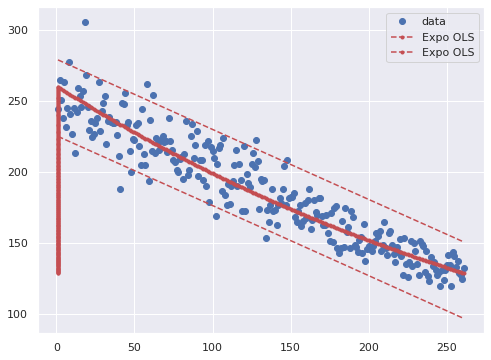
\includegraphics{analise-de-dados/regressao/regressao_EXPO.png}
    \caption{Regressão Exponencial para os tempos de espera}
    \label{fig: plot_Expo_OLS}
\end{figure}

\begin{figure}[H]
    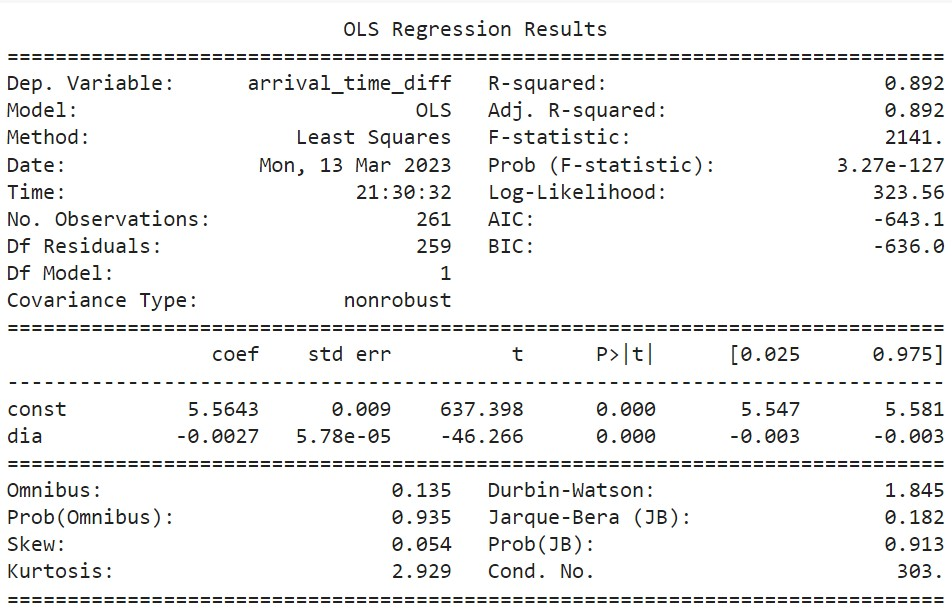
\includegraphics[scale = 0.85]{analise-de-dados/regressao/EXPO_OLS_Summary.jpg}
    \caption{Resumo da regressão}
    \label{fig: sum_Expo_OLS}
\end{figure}

Para Este caso, a explicabilidade do modelo aumentou e o problema que antes existia já não mais existe. Como os Valores P seguem menores do que 0, o modelo existe e pode ser usado.


\section{Conclusão}
A análise de dados foi um importante processo para o projeto de simulação que está sendo desenvolvido. Por meio dela conseguimos compreender, e testar, quais os melhores níveis de agregação, as distribuições que melhor representam os dados do projeto, o comportamento dos parâmetros e as tendências sob as quais estes se apoiam. Dessa forma, foi possível definir o nível de agregação mensal para o planejamento das atividades do call center, por ser o nível que melhor representa o crescimento do número de chegadas ao longo do ano, assim como modelar os tempos de serviço para o ano inteiro.

Restam como etapas a modelagem dos processos a serem simulados, bem como dos dados que estes receberão durante a simulação. Em especial, a dos tempos entre chegadas, que são não estacionários e, por consequência, são melhor representados por um processo de Poisson ou algum outro método que leve em consideração o tempo decorrido na simulação. Desta maneira, esse será um dos futuros esforços do projeto.

Outros desses esforços serão incluir o processo de tendência na simulação e na tomada de decisão para o cliente, garantindo uma assertividade maior ao projeto. Afinal, é esperado que o problema apresentado volte a ocorrer no tempo se a solução oferecida apenas resolva o estado presente do sistema.

\end{document}